\chapter{Alternative systemer}
\label{Comparison}
Udover at udvikle vores udgave af et booking-system til IT-Universitetet, vil vi i dette kapitel give en kort beskrivelse af to alternative  systemer og sammenligne dem med vores løsning.

\section{Room Booking System}
\label{Comparison_RBS}
"Room Booking System"\footnote{http://www.roombookingsystem.co.uk/} er et web-baseret bookingsystem designet til både skoler og virksomheder. 

Brugergrænsefladen er designet som en kalender, hvor man kan vælge hvilke kategorier af resurser, man kan vil se tider for: for eksempel IT rum, mødelokaler, projekter eller andet udstyr. Bookinger af diverse resurser er, ligesom vores system, opgjort i farvekoder, så man hurtigt kan få et overblik over, hvad der er ledigt og hvad der er booket. Figur \ref{Comparison_RBS_RoomBookingSystem} viser det første skærmbillede i "Room Booking System".

\begin{figure}[h!]
  \centering
    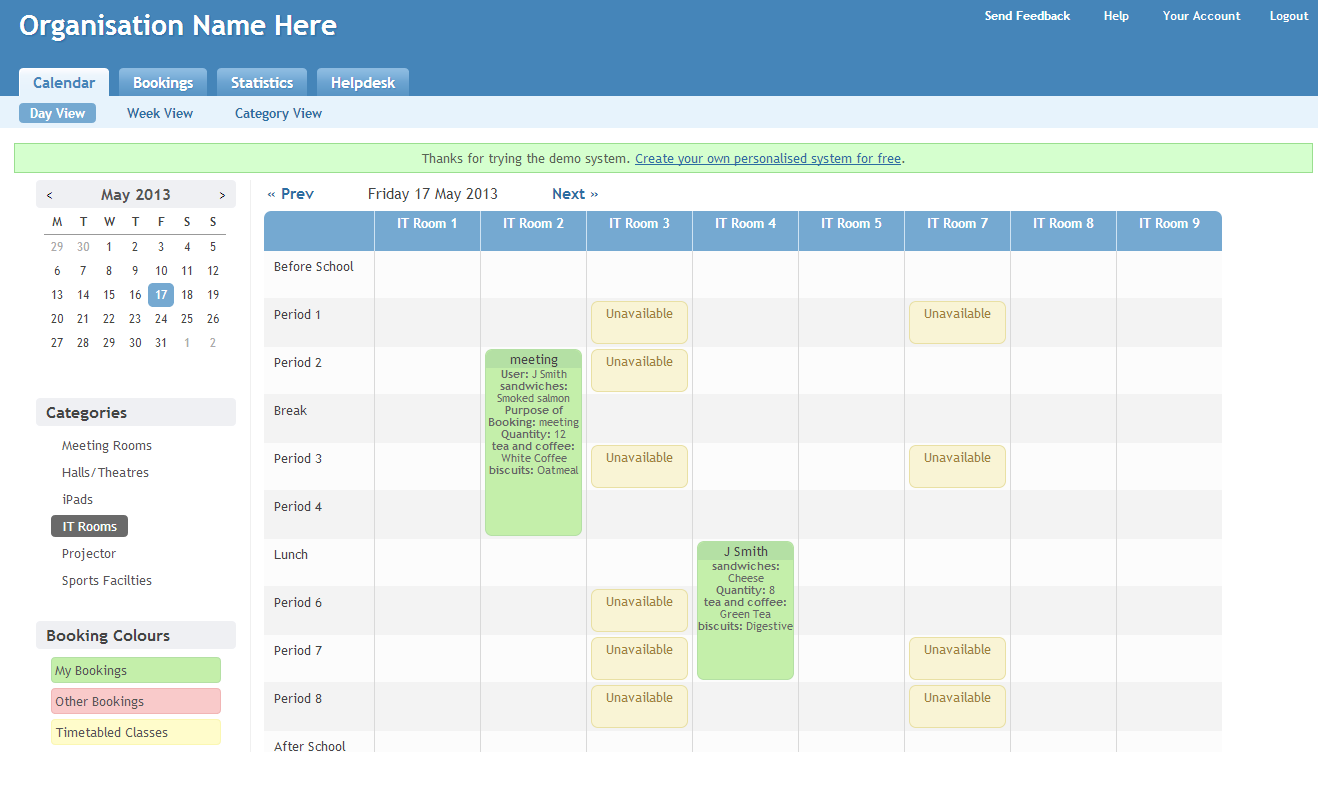
\includegraphics[width=0.8\textwidth]{Appendix/GUI-Prototype/RoomBookingSystem}
  \caption{Det første skærmbillede i systemet, som viser oversigten over bookede resurser}
\label{Comparison_RBS_RoomBookingSystem}
\end{figure}

"Room Booking System" giver også mulighed for tilføje forplejning til ens bookinger. Figur \ref{Comparison_RBS_RoomBookingSystemList} viser skærmbilledet, der svarer til vores booking-liste. Her kan det ses, at der til bookingen er blevet bestilt sandwicher med røget laks plus te og kiks.

\begin{figure}[h!]
  \centering
    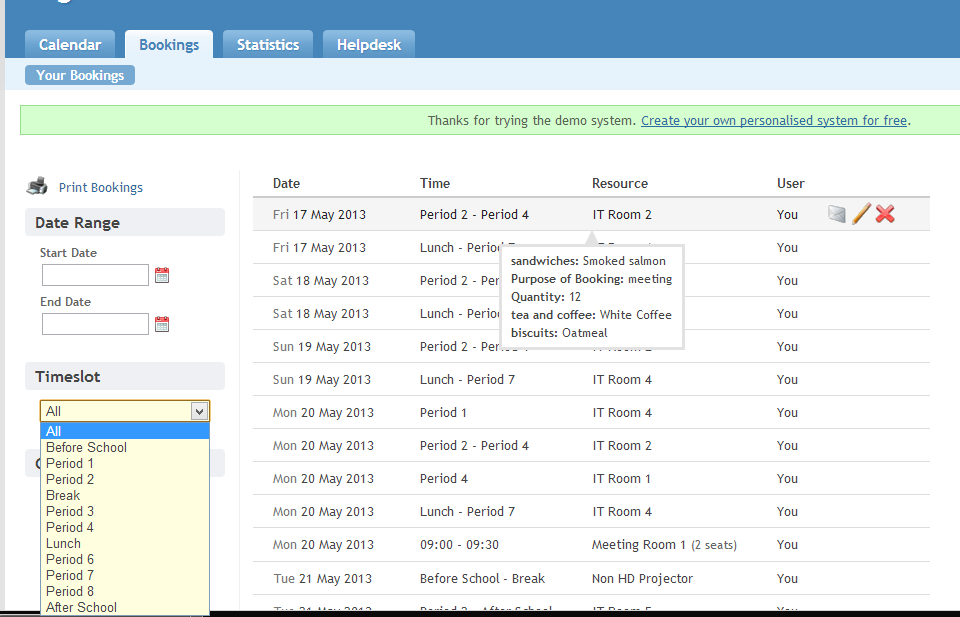
\includegraphics[width=0.8\textwidth]{Appendix/GUI-Prototype/RoomBookingSystemList}
  \caption{Skærmbillede over de bookinger, der er i systemet}
\label{Comparison_RBS_RoomBookingSystemList}
\end{figure}

Desuden er login til systemet separat og dermed er der ikke mulighed for at integrere det med hverken Active Directory (AD). Et abonnement, der understøtter 200 lokaler/udstyr og 500 brugere, koster $\sim$434 kr. om måneden.

En fordel ved "Room Booking System" er, at det giver mulighed for at lave statistikker (figur \ref{Comparison_RBS_RoomBookingSystemStatistic}). Desuden kan det ses som en fordel, at det er hostet eksternt.

\begin{figure}[h!]
  \centering
    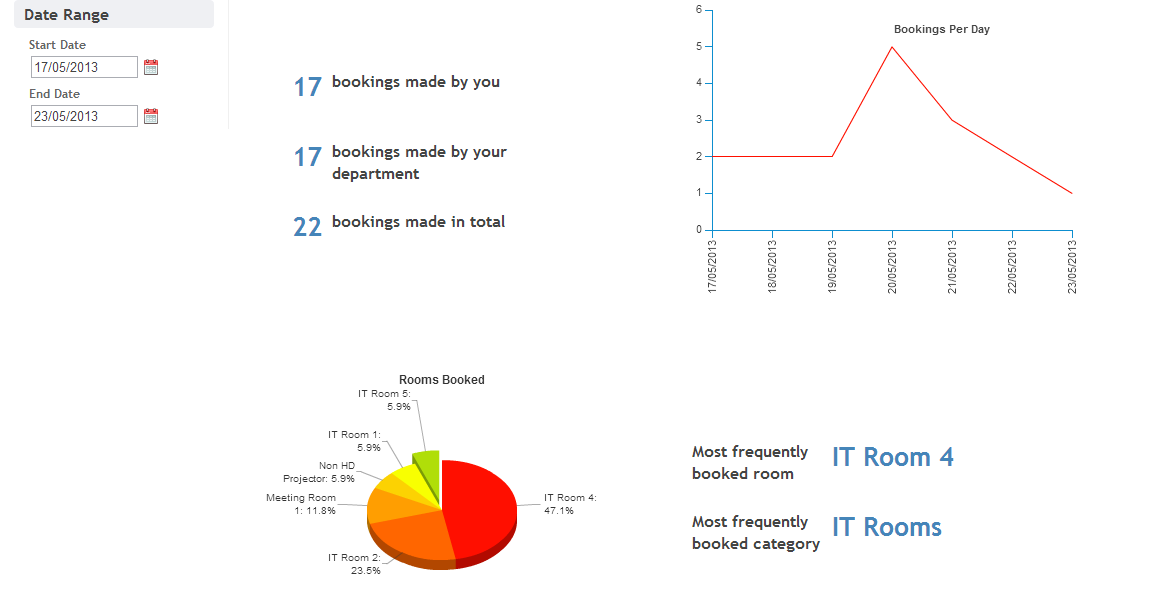
\includegraphics[width=0.8\textwidth]{Appendix/GUI-Prototype/RoomBookingSystemStatistic}
  \caption{Skærmbillede til visning af statistik over booking af resurser.}
\label{Comparison_RBS_RoomBookingSystemStatistic}
\end{figure}

Vi vurderer, at brugervenligheden i "Room Booking System" er lidt dårligere end i vores, da der er flere skærmbilleder. Udover det er der ikke synderlige problemer i forhold til brugervenlighed.

Ulempen ved "Room Booking System" (i forhold til vores løsning) er, at der er en grænse for hvor mange lokaler og udstyrselementer, som kan bookes i systemet. Desuden er det ikke muligt at integrere med et eksisterende ITU login system. Da der kun er mulighed for 500 brugere i systemet, vil nogle brugere skulle slettes for, at der kan oprettes nye brugere i forbindelse med nye studerende/ansatte.

\section{School Booking}
\label{Comparison_SB}
"School Booking"\footnote{http://www.schoolbooking.com/} er et andet web-baseret system, som primært er designet til brug af skoler. 

Systemet giver mulighed for at booke både lokaler og udstyr\footnote{Det bookede udstyr kan være forplejning, hvis man sætter det rigtigt op.}. Man kan betale ekstra for at tillade eksterne bookere. Statistik er også muligt i dette system. Der er dog ikke mulighed for at integrere det med Active Directory.

Et system, der understøtter 1000 brugere, 300 lokaler/resurser, eksterne bookere og statistik koster årligt $\sim$11.500 kr.

Fordelen ved dette system er det samme som ved "Room Booking System": muligheden for at lave statistik.

Ulempen ved dette system er, at der er en begrænset mængde af brugere, som kan anvende systemet, samt at det ikke er muligt at integrere det med AD eller lignende, fordi det er hostet eksternt.

Vi har desværre ikke haft mulighed for at undersøge brugervenligheden af systemet, da der ikke var nogen tilgængelige skærmbilleder.  Det var heller ikke muligt for os at afprøve systemet, da det krævede, at man skulle være en registreret bruger for, at man kunne prøve deres 30 dages prøveperiode.